\cotefile{67}
\scanpage{69}
des syst. admissibles de disques \inserted{conformes} autour
des $a_i$, vers l'ens des syst.
de disques \deleted{conformes} \inserted{\deleted{\unsure{secto|vecto}} standards} dans les $T_{X,a_i}$,
est bijective. \deleted{Au niveau des
\unsure{esp.|espaces}} Au niveau des espaces
modulaires de type Teichmüller,
cela donnerait donc une \deleted{\unsure{iso|is|la}} structure
de fibré principal \deleted{$TB_{g,I}\mathrel{\unsure{\sim|\to|\xrightarrow{\sim}}}T_{g,\nu}$} de groupe
structurel $(\mathbb{R}^{\times+})^I$ : $TB_{g,I}$
sur $T_{g,I}$ $(\operatorname{Card}I=\nu)$, \deleted{\unsure{ce}}

\deleted{\unsure{en passant aux log})} Si la\deleted{\unsure{dé|dès}} \unsure{veléité|velléité|relation} qui précédait
\deleted{la conjecture} était vraie, cel signifierait
qu'on aurait une section canonique
de ce fibré, ce qui implique
aussi que pour un $\mathrm{p}^{\mathrm{t}}$ de $T\deleted{B}_{g,I}$,
i.e. une surface hol \inserted{ponctuée} ($X_0$-rigidifiée)
de type $(g,\nu)$, il y aurait un syst.
d'ouverts can. ds les $T_{X,a_i}$, i.e. des
% archive sheet number: 71

\scanpage{70}
\mspage{9}
métriques euclidiennes \uline{canoniques} sur
les $T_{X,a_i}$, décrivant leur structure
conforme. Dans le cas $g\geq 2$ et $=$
encore pour $g=1$, cela ne semble pas
inquiétant, puisqu'on a une
métrique canonique sur $X$. Par
contre dans le cas $g=0$, cela semble
étrange, puisque dans ce cas on n'a
\uline{pas} de métrique canonique sur $X$.

\uline{12.1.}

5. \uline{Retour sur le principe de chirurgie conforme}

La formulation des lemmes \inserted{locaux} 2 et 3, qui
sont l'ingrédient technique essentiel pour le
th. 4 (et lui sont équivalents), est un peu
alambiquée. Il est plus élégant de se
réduire à des lemmes globaux de type
uniformisation par le disque $\mathbb{D}$. Cela
donne le
% archive sheet number: 72

\scanpage{71}
\uline{Lemme 4}

% slanted
\margin{\uline{NB} Il y a une version plus faible de A), où $\dot U=C$ (sans $I$), qui n'est pas formellement contenue ds A).}

A) Soit $U$ une partie ouverte bornée
de $\mathbb{C}$, dont la frontière est \inserted{réunion de} une
courbe de Jordan \deleted{rectifiable. Alors
il existe une \unsure{fonction,|fonction} continue
$f:\mathbb{D}\longrightarrow$}
$C$, et d'un \deleted{homéomorphisme} intervalle
topologique $I$ tel que
$I\cap C=\{b\}$, \deleted{\unsure{et}} (alors $I\setminus\{b\}$ est
contenu dans la comp. connexe
bornée $V$ de $\mathbb{C}\setminus C$, et $b$
est une extrémité de $I$, \inserted{notons $U=V\setminus I'$, où $I'=I\setminus\{b\}$}). \deleted{Soit} On
suppose de plus que $C$ et $I$ soient rectifiables.
Soit $a$ l'autre extrémité de $I$. Alors il
existe une fonction \deleted{continue} $f:\mathbb{D}\longrightarrow\mathbb{C}$
telle que

\figure{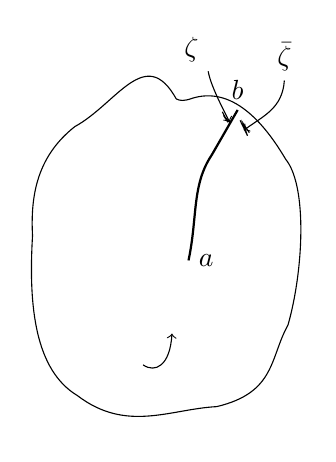
\begin{tikzpicture}[x=.78cm,y=.78cm]
\draw (0,2.1) .. controls (-.5,3) and (-.97,2.02) .. (-1.65,1.65) .. controls (-2.3,1.14) and (-2.37,.46) .. (-2.34,-.13) .. controls (-2.41,-1.30) and (-2.29,-2.32) .. (-1.61,-2.73) .. controls (-.81,-3.34) and (-.10,-2.95) .. (.66,-2.91) .. controls (1.62,-2.68) and (1.52,-2.12) .. (1.82,-1.58) .. controls (2.07,-.70) and (2.14,.68) .. (1.78,1.12) .. controls (1.35,1.85) and (.84,2.29) .. (.26,2.11) .. controls (.12,2.06) and (.06,2.07) .. (0,2.1);
\draw[thick] (.2,-.53) node[right]{$a$} .. controls (.35,.18) and (.25,.7) .. (.58,1.19) -- (1,1.92) node[above]{$b$};
\draw[->] (.52,2.55) node[above left]{$\zeta$} .. controls (.56,2.32) and (.75,1.96) .. (.87,1.72);
\draw[->] (1.76,2.40) node[above]{$\bar\zeta$} .. controls (1.73,1.94) and (1.41,1.82) .. (1.10,1.59);
\draw (.75,1.89) -- (.84,1.72) -- (.77,1.83) -- (.88,1.71);
\draw (1.04,1.75) -- (1.16,1.50) -- (1.09,1.70) -- (1.19,1.55);
\draw[->] (-.54,-2.23) .. controls (-.34,-2.37) and (-.10,-2.24) .. (-.07,-1.72);
\end{tikzpicture}}

1) $f$ est continue, et induit une \deleted{ho} bijection
(voire un homéo !) $\mathring{\mathbb{D}}\xrightarrow{\sim}U$.

2) $f(\zeta)=f(\bar\zeta)=b$, et $f$ induit une bijection
(voire un homéo) $\deleted{\alpha}\inserted{\alpha\setminus\{\zeta\bar\zeta\}}\xrightarrow{\sim} C\setminus\{b\}$.
(NB $\zeta=\exp 2i\pi/3$, et $\alpha,\beta,\bar\beta$ sont les trois
arcs sur $\partial\mathbb{D}$ déterminés par $1,\zeta,\bar\zeta$).

\figure{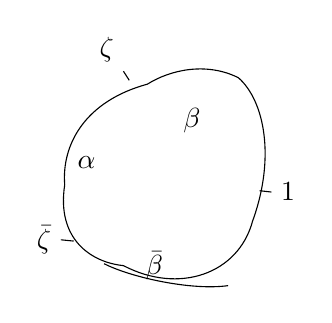
\begin{tikzpicture}[scale=.82]
\draw (1.1,1.4) .. controls (.6,1.65) and (.04,1.52) .. (-.31,1.30) .. controls (-1.27,1.04) and (-1.64,.37) .. (-1.59,-.26) .. controls (-1.72,-1.10) and (-1.18,-1.46) .. (-.68,-1.51) .. controls (.18,-1.96) and (1.1,-1.64) .. (1.32,-.82) .. controls (1.68,.17) and (1.50,1.05) .. (1.1,1.4);
\draw (-.59,1.36)--(-.68,1.50) node[above left]{$\zeta$};
\draw (-1.45,-1.13)--(-1.65,-1.11) node[left]{$\bar\zeta$};
\draw (1.43,-.35)--(1.61,-.37) node[right]{$1$};
\node at (-1.25,.09){$\alpha$};\node at (.38,.74){$\beta$};\node at (-.20,-1.51){$\bar\beta$};
\draw (-.98,-1.48) .. controls (-.57,-1.69) and (.37,-1.90) .. (.94,-1.82);
\end{tikzpicture}}

3) $f\mid\beta$ et $f\mid\bar\beta$ induisent des bijections de
$\beta$ et $\bar\beta$ sur $I$). NB a) b) c) peuvent
s'exprimer en disant que $f$ induit un
\deleted{\unsure{isom}} \inserted{homéo} de $\mathbb{D}$ sur le découpé de $\bar U=\bar V$
suivant $I$ (ou sur $I\cup C=\dot U$).

4) $f\mid\mathring{\mathbb{D}}$ est holomorphe.
% archive sheet number: 73

\scanpage{72}
\mspage{10}
\uline{NB 1} Cette fonction est unique, dû au fait
que \deleted{\unsure{les|le}} le groupe des automorphismes \deleted{conformes}
holomorphes de $\mathbb D$ agit de façon simplement
transitive sur l'ens des
triples \deleted{\unsure{d'él.|ord}} de pts distincts $(r,s,t)$ \inserted{sur $\mathbb{S}^{1}=\partial\mathbb D$} qui se
suivent pour l'orientation canonique de
$\deleted{\partial\mathbb D}\mathbb S^1$. \deleted{\unsure{D'où|Donc} \unsure{il}}

\uline{NB 2} La condition 3) implique qu'on a un
\unsure{homéo|bijection} canonique
\[
\varphi:\beta=(\widehat{1,\zeta})\simeq\bar\beta=(\widehat{1,\bar\zeta})
\]
tel que $\varphi(1)=1$, $\varphi(\zeta)=\bar\zeta$).

B) Cette application $\varphi$ est rectifiable. Inversement,
\deleted{toute} tout \deleted{application} \inserted{homéo} rectifiable $\varphi:\beta\xrightarrow{\sim}\bar\beta$
provient d'une situation comme en A.
De façon plus précise, \deleted{on peut \unsure{supp.} \inserted{\deleted{il existe}}}
(quitte à remplacer $\bar V$ par $\mathbb D$ par le th. d'uniformisation A)
simplifié sans segment intérieur $I$,
et normaliser la situation en \deleted{\unsure{plaçant|plaçan}} ramenant
$a$ en $0$, $b$ en $1$) \deleted{il existe \unsure{un|une}} Il existe
une application continue
\[
f=f_\varphi:\mathbb D\mathrel{\unsure{-|\to}}\mathbb D
\]
telle que

1) $f\mid\mathbb D^\circ$ soit \deleted{holo} injection holomorphe
% archive sheet number: 74

\scanpage{73}
(soit $U=f(\mathbb D^\circ)$)

\figure{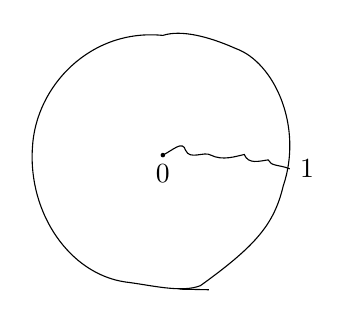
\begin{tikzpicture}[scale=.76]
\draw (0,2) .. controls (-1.20,2.12) and (-2.13,1.16) .. (-2.18,.12) .. controls (-2.25,-.96) and (-1.57,-1.98) .. (-.63,-2.12) .. controls (-.21,-2.17) and (.32,-2.31) .. (.63,-2.18) .. controls (1.56,-1.51) and (1.86,-1.15) .. (2.01,-.52) .. controls (2.35,.48) and (1.86,1.55) .. (1.22,1.78) .. controls (.77,1.98) and (.31,2.10) .. (0,2);
\draw (0,0) .. controls (.18,.09) and (.33,.25) .. (.38,.08) .. controls (.45,-.09) and (.69,.07) .. (.80,0) .. controls (1,-.10) and (1.22,-.02) .. (1.36,.01) .. controls (1.43,-.16) and (1.61,-.10) .. (1.76,-.08) .. controls (1.80,-.19) and (1.96,-.16) .. (2.12,-.23);
\fill (0,0) circle (.038) node[below]{$0$};\node[right] at (2.13,-.23){$1$};
\draw (.28,-2.24)--(.77,-2.25);
\end{tikzpicture}}

2) $f(0)=0$, $f(\zeta)=f(\bar\zeta)=1$
\deleted{3) $f\mid\unsure{\beta|\alpha}$ est un}
$f\mid(\alpha\setminus\{\zeta,\bar\zeta))$ \deleted{est} \inserted{induit} un
homéo avec $\partial\mathbb D\setminus\{1\}$

3) $\deleted{f\mid[1,\zeta\mathclose{\unsure{[|]}}}$ $f\mid\beta$ et $f\mid\bar\beta$ sont injectives et
ont $=$ image, \deleted{qui \unsure{est|contient}, et $I\setminus\{1\}$} \inserted{$I$, contenant $\{1\}$} d'après
2) et $I\setminus\{1\}$ est contenu dans $\mathbb D^\circ$.

4) Soient $f_1:\beta\xrightarrow{\sim}I$, $f_2:\bar\beta\xrightarrow{\sim}I$ induits par $f$,
\inserted{alors $\varphi=f_2^{-1}f_1$}

\uline{NB} Ici encore, $f$ est unique. On peut
résumer ce théorème d'uniformisation
avec bord dans le \deleted{Scholie}

\uline{Scholie} Il y a corr. 1-1 entre les
données suivantes :

a) Les homéos rectifiables \deleted{\unsure{croi}}
\[
\begin{aligned}
\psi:[0,1]\simeq[0,1] &\qquad\text{avec }\psi(0)=0\\
&\qquad\text{donc }\psi(1)=1
\end{aligned}
\]

b) Les segments topologiques \uline{rectifiables}
$I$ dans $\mathbb D$, tels que \deleted{$I\cap\partial\mathbb D$ soit réduit
à une extrémité de $I$} \inserted{$I$ admette $0,1$ comme}
extrémités et \deleted{$I\setminus\{1\}\unsure{\subset|=}\unsure{1}$}
$I\cap\partial\mathbb D=\{1\}$ (i.e.
$I\setminus\{1\}\subset\mathbb D^\circ\}$

c) Les \deleted{\unsure{ap}} applications continues $f:\mathbb D\mathrel{\unsure{-|\to}}\mathbb D$
qui ont les propriétés 1) 2) 3) de B) ci-dessus
% archive sheet number: 75

\scanpage{74}
\mspage{11}
d) Les séries convergentes
\[
f=\sum_{i\geq0}a_i z^i\qquad(a_i\in\mathbb C)
\]
de rayon de convergence $\geq1$ (donc
définissant $\mathbb D^\circ\mathrel{\unsure{-|\to}}\mathbb C$) \inserted{avec $|f(z)|\leq1$ si $z\in\mathbb D$,} telles que la $f$
se prolonge par continuité en une
fonction $\mathbb D\mathrel{-}\deleted{\mathbb C}\mathbb D$, celle-ci ayant les
propriétés 1) 2) 3) de B) ci-dessus.

\uline{13.1.}\qquad\textcircled{6}

Soit $(X,C)$ un objet du groupoïde
de Teichmüller analytique complexe
à bord, avec la condition différentiable.
Pour fixer les idées, supposons $X$ connexe,
de type $g,\nu$. Considérons le découpé $X'$
de $X$ suivant $C$, bouchons ses trous \inserted{canoniquement en utilisant la structure torique de $\partial X'$, $*$}
% slanted
\margin{$*$ via la métrique riemannienne can. de $X'$}
d'où surface holomorphe compacte \inserted{sans bord $X''$}, à disques
\inserted{pointés} marqués, avec des \deleted{iso} \inserted{antiiso} de \deleted{ces} \inserted{certains de ces} disques
(\deleted{deux à deux} qui se groupent par paires, à l'exception
des $\nu$ disques correspondant à $\partial X$).

On peut considérer $X''$ comme le
normalisé d'une courbe \deleted{\unsure{alg}} \inserted{$\mathbb C$-alg $X'''$} ``stable''
(au sens de Mumford-Deligne), en
% archive sheet number: 76

\scanpage{75}
identifiant les pts des centres des disques
qui se correspondent, et en ponctuant
par les centres des autres disques.
De plus, on obtient, \deleted{\unsure{un|une}} pour chaque
point singulier $x$ de $X'''$, correspondant
à une paire $\{x_1,x_2\}$ de points de
$X''$ (centres des deux disques associés),
grâce à l'antiisomorphisme de ces
disques pointés, un élément \inserted{non nul} \deleted{de} (i.e. une base)
de
\[
T_{X'',x_1}\underset{\mathbb C}{\otimes}T_{X'',x_2}
\]
i.e. \deleted{\unsure{de|un}} élément de
\[
T_{X'',x_1}^{*}\mathbin{\wedge}_{\mathbb C^*}T_{X'',x_2}^{*}.
\]

On trouve ainsi un foncteur de

a) Catégorie \inserted{(groupoïde)} des courbes hol. cptes à bord \inserted{$X$} de
type $g,\nu$, avec découpage holomorphe
(avec comme flèches les iso)

vers

b) Catégorie des courbes \inserted{$\mathbb C$-alg} stables de type $(g,\nu)$
$X'''$, munies \inserted{1°)} d'une ``structure de propagation
normale'' en ses pts singuliers, et 2°) d'un
\deleted{structure de multidisques} \inserted{syst.} admissible de
disques autour des pts marqués.
% archive sheet number: 77

\scanpage{76}
\mspage{12}
Au niveau des multiplicités modulaires \inserted{(analytiques réelles)},
on trouve sûrement un morphisme pour
celles-ci
\[
\begin{aligned}
&\deleted{MB_{g,\nu}\unsure{-|\to}}\\
&MDB_{g,\nu}\longrightarrow M_{\mathrm{st}}N\deleted{{}_{g,\nu}}D_{g,\nu}
\end{aligned}
\]
où $MDB_{g,\nu}$ désigne la multiplicité modulaire
($M$) pour les surfaces holomorphes compactes
``découpées'' ($D$) à bord ($B$) de type $g,\nu$, et
$M_{\mathrm{st}}ND_{g,\nu}$ celle pour les courbes algébriques
stables (de type loc. constant) \inserted{de type $g,\nu$} à structure de
propagation normale ($N$) et à système \inserted{adm} de
disques ($D$) autour des pts marqués.

Cette flèche est compatible avec les
flèches canoniques vers la cat. des
types combinatoires \inserted{-toriques} de tels objets
(diagrammes $MD$ (Mumford-Deligne ou
``modulaires'') (\deleted{avec pond} \inserted{incluant} une pondération
des sommets) à structures toriques
associées aux arêtes\ldots{} donnant lieu un
diagramme commutatif
% archive sheet number: 78

\scanpage{77}
\diagram{\begin{tikzcd}[ampersand replacement=\&,column sep=small]
MDB_{g\nu}\arrow[rr,dash,"{\unsure{-|\to}}" description,near end]\arrow[dr]\& \& M_{\mathrm{st}}ND_{g,\nu}\arrow[dl]\\
\& mdt_{g,\nu}\&
\end{tikzcd}}

(dans $mdt$, la lettre $t$ rappelle qu'on a inclus
des structures toriques dans le type
combinatoire). Sûrement aussi, si on
\deleted{définit} \inserted{considère} $MD_{g,\nu}$ (sans bord, ou à bord
``généralisé'' réduit à un ens de $\nu$ pts)
et $M_{\mathrm{st}}N\deleted{D}_{g,\nu}$ (sans structure \inserted{multi}disque) on
aura

\diagram{\begin{tikzcd}[ampersand replacement=\&,column sep=small]
MD_{g,\nu}\arrow[rr]\arrow[dr]\& \& M_{\mathrm{st}}N_{g,\nu}\arrow[dl]\\
\& md_{g,\nu}\&
\end{tikzcd}}

cette fois un morphisme de \deleted{\unsure{cl|de}}
multiplicités \deleted{\unsure{analyti|analytiques}} $\mathbb C$-algébriques.
Dans le cas 1), les dimensions \inserted{(réelles)} de
part et d'autre sont celles de $\mathbb C^{\unsure{3|6}g-3+\nu}\times\mathbb R^\nu$,
\inserted{les dims. complexes} dans le cas 2), \inserted{sont} celle de $\mathbb C^{3g-3+\nu}$.
% archive sheet number: 79

\scanpage{78}
\mspage{13}
\uline{Question} Ces flèches sont elles des iso
\deleted{\unsure{--}} et si oui, comment expliciter un
iso en sens inverse ? \deleted{Si}

Si la détermination conjecturale des
syst. admissibles de disques sur une
surface holomorphe \inserted{compacte} ponctuée (de type
hyperbolique) était correcte, on trouverait aisément
\deleted{des \unsure{foncteurs}} \inserted{flèches} en sens
inverse; Au niveau plus naïf des
foncteurs (entre les catégories-sections
de ces multiplicités) on trouverait
ceci : à l'aide d'un \deleted{\unsure{iso}}
\[
u_i\in T_{x'_i}^{\times}\wedge_{\mathbb C^\times}T_{x''_i}^{\times}
\]
ou ce qui revient au $=$, un
\[
w_i(=u_i^{-1})\in T_{x'_i}^{\vee\times}\wedge T_{x''_i}^{\vee\times}
\]
\deleted{choisissant \unsure{iso}} \inserted{i.e. un} ``accouplement dualisant''
\[
\deleted{T_{x'_i}^{\vee}\xrightarrow{\sim} T_{x''_i}}\quad T_{x_i}\otimes T_{x''_i}\longrightarrow\mathbb C
\]
choisissant un \deleted{\unsure{métriq}} disque conforme
$D'_i$ de $T_{x'_i}$, \deleted{\unsure{on en déd}} d'où disque
conforme polaire $D''_i$ de $T_{x''_i}$, on
trouverait \deleted{des} pour ce syst. $(D'_i)$ $(D''_i)$
des réalisations de ces disques comme
% archive sheet number: 80

\scanpage{79}
plongés dans $X''$ normalisé de $X'''$ \deleted{dont} \inserted{avec lequel} on part, et \deleted{on} trouver des antiiso entre les bords \deleted{de ces} de $D'_i,D''_i$ -- d'où possibilité de recoller pour trouver une $X$ surface hol à bord, si on a aussi enlevé des disques ouv. $\mathring D_{\alpha}^{\unsure{*|k}}$ correspondants aux pts marqués $x_{\alpha}$, sinon une surface à pts marqués), découpée par des cercles $\Gamma_i$ qui ne sont \deleted{pas} \inserted{peut-être pas} néc. géodésiques \deleted{(\unsure{ce sera}} \inserted{(?? à} examiner de plus près) mais définissent des cercles géodésiques uniques, par les principes de Thurston.

Il faudrait voir que le résultat obtenu ne dépend pas des choix des paires $(D'_i,D''_i)$ mut.\textsuperscript{t} polaires, il y a un argument heuristique pour cela tout à fait vaseux, consistant à dire qu'une petite variation de \unsure{cette,|cett,}
% archive sheet number: 81

\scanpage{80}
\mspage{14}
paire ne change rien; car si on remplace $D'_i$ par $\lambda D'_i$, donc $D''_i$ par $1/\lambda\,D''_i$, avec $\lambda\in\mathbb R^{*+}$ voisin de $1$, les \unsure{mêmes|dites|trois} relations \unsure{vaudront|voudront} \unsure{pour|fixer} les disques obtenus dans \inserted{le normalisé} $X''$ (c'est probablement tout à fait faux !), et on obtiendrait la $=$ surface recollée $X$ mais les $\Gamma_i$ remplacés par des cercles ``voisins'' $\Gamma'_i$.

Le cas-clef à comprendre sans doute est celui où $(g,\nu)=(0,4)$, i.e. le mécanisme de recollement de deux ``pantalons'' de Thurston, donc pour \deleted{\unsure{un ens}} \inserted{deux} ens$'$ $\unsure{\mathscr E|E|\Sigma}',\mathscr E''$ à deux éléments, fixés, les \unsure{foncteurs|fonctions|fonction} des
\[
\left\{\begin{aligned}
&\text{pantalons de types combinatoires } E'\amalg\{s\},\ E''\amalg\{t\},\\
&\text{recollés suivant } \{s,t\},\ \text{\deleted{donné} suivant}\\
&\text{les données }(l_i)_{i\in E'\amalg E''\amalg u}\in(\mathbb R^{*+})^{E'\amalg E''\amalg u},\\
&\text{et }\theta\in\mathbb U_{E'\wedge E''}\text{ qui fixe le recollement}
\end{aligned}\right.
\]
vers
% archive sheet number: 82

\scanpage{81}
\[
\left\{\begin{aligned}
&\text{paires de pantalons \deleted{\unsure{dég|dégé}} généralisés \inserted{$X',X''$ à \unsure{trous|bord}}, indexés}\\
&\text{par }E'\amalg\{s\},\ E''\amalg\{t\},\ \text{avec }s,t\text{ correspondant}\\
&\text{aux \deleted{bords} composantes ponctuelles du}\\
&\text{bord, avec les paramètres }(\lambda_i)_{i\in E'\amalg E''}\in\mathbb R^{\unsure{*+E'\amalg E''|\Sigma'\amalg\Sigma''}},\\
&\text{et un isom d'identification}\\
&\text{dans }\mathbb C^*\wedge_{\pm1}(E'\wedge E'')
\end{aligned}\right.
\]

Une fois ce cas compris, et revenant alors au cas général, il faudrait déjà, pour un type de découpage donné incarné par un diagramme $\mathrm{MD}$ du $md_{g,\nu}$, comprendre l'application sur les groupes fondamentaux induite par
\[
\mathrm{MDB}_{\unsure{g}}\longrightarrow \mathrm M_{\mathrm{st}}\mathrm{ND}_{g,\nu}, \tag*{($*$)}
\]
celui des deuxièmes membres étant essentiellement compris en termes de groupes de Teichmüller spéciaux -- \uline{mais il doit en être pareil pour les premiers} ! Également, il ne devrait pas être bien dur de vérifier si ($*$)
% archive sheet number: 83

\scanpage{82}
\mspage{15}
est étale, en calculant i.e. interprétant son application tangente.
% archive sheet number: 84

\scanpage{84}
\uline{\unsure{Modulis|Modulus} $M_{0,4}$ et l'octaèdre}

$I$ ens de card. $4$ d'où

$J=\mathscr P_{2,2}(I)$, $V(J)$ plan vectoriel sur $\mathbb F_2$ avec $V(J)^*\simeq J$,

$V(J)\subset\unsure{\mathfrak S|\mathfrak G}_I$ formé de l'identité et des ``bitranspositions''.

On s'intéresse aux droites projectives (sur $\mathbb C$ disons -- ça marcherait sur tt corps alg clos \inserted{de car. $\ne2$}) munies de $I\hookrightarrow X$. (plus précisément $I_{\mathbb C}\hookrightarrow X$, ou $I\to X(\mathbb C)$ ...).

L'opération de $V(J)$ sur $I$ se prolonge en une opération de $V(J)$ sur $X$
\[
V(J)\hookrightarrow G_X=\operatorname{Aut}(X)
\]

Soit \qquad $S=$ ens des pts de $X$ qui sont fixes par un élément de $J=V(J)^*$
\[
\text{d'où}\qquad \operatorname{card} S=6
\]

% slanted
\margin{\uline{\unsure{Commencer}} \uline{par Ça !}}
En fait, on trouve que \deleted{\unsure{pour tt}} \inserted{les} opérations \deleted{de} \inserted{fidèles} d'un plan vectoriel $V$ sur un $X$, i.e les plongements $V\deleted{\unsure{(J)}}\subset G_X$, sont tous équivalents (modulo autom intérieurs de $G_X$) et sont (pour une base fixée \inserted{$e_0,e_1$}) équivalents à l'opération sur $\mathbb P^1$
\[
\begin{aligned}
u(e_0)&=(z\longmapsto-z)=\begin{pmatrix}-1&0\\0&1\end{pmatrix}&&\text{pts fixes }0,\infty\\
u(e_1)&=(z\longmapsto1/z)=\begin{pmatrix}0&1\\1&0\end{pmatrix}&&\text{pts fixes }\pm1\\
u(e_0+e_1)&=(z\longmapsto-1/z)=\begin{pmatrix}0&-1\\1&0\end{pmatrix}&&\text{pts fixes }\pm i
\end{aligned}
\]

Les \deleted{\unsure{groupes gén}} \inserted{sous groupes} isom. à $D_2$ de $G_X$ correspondent $1$-$1$ aux parties $S$ de cardinal $6$ de $X$, isom. à $(\mathbb P_1,\{0,\infty,\pm1,\pm i\})$.
% slanted
\margin{parties octaédrales d'une droite projective}

Le normalisateur d'un tel \deleted{$D_2$} sous groupe $V$ \inserted{dans $G_X$} est isomorphe au groupe \deleted{des autom} $\mathfrak S_4$ (de façon non canonique), plus précisément, si $V=V(J)$ avec $J=\unsure{J|V|\mathfrak P}(I)$, \inserted{i.e. si $I$ est un $V$-torseur}, on trouve \inserted{alors} iso de suites exactes
\diagram{\begin{tikzcd}[ampersand replacement=\&]
\& \& \deleted{\unsure{\operatorname{Aff}(V)}} \arrow[d,equal] \& \& \\
1\arrow[r] \& V\arrow[r]\arrow[d,equal] \& \mathfrak S_I\arrow[r]\arrow[d] \& \operatorname{Aut}(V)\arrow[r]\arrow[d,equal] \& 1\\
1\arrow[r] \& V\arrow[r] \& \Gamma\arrow[r] \& \operatorname{Aut}(V)\arrow[r,dash] \& 1
\end{tikzcd}}
défini modulo autom intérieurs par un élément de $V$. Quand $I$ est le torseur trivial, se donner un tel \deleted{\unsure{iso}} iso d'ext.
% archive sheet number: 86

\scanpage{85}
revient à se donner un scindage de l'extension
\diagram{\begin{tikzcd}[ampersand replacement=\&,column sep=small,row sep=tiny]
(*) \& 1\arrow[r] \& V\arrow[r] \& \Gamma\arrow[r]\arrow[d,equal] \& \underline{\operatorname{Aut}(V)}\arrow[r] \& 1\\
\& \& \& \operatorname{Nor}_{G}(V) \& \simeq\unsure{\mathfrak S|\mathfrak G}_{J} \&
\end{tikzcd}}

En termes géométriques, ces scindages sont associés aux quatre systèmes de \inserted{paires de} faces antipodiques sur l'octaèdre. \deleted{\unsure{Ainsi, les|Ainsi les}} L'octaèdre combinatoire (non orienté a priori) se définit à partir de l'ens $S$ de ramification, et l'antipodisme \deleted{sur} $S$, de la façon habituelle; ses faces sont les parties à trois éléments \deleted{qui} $S'$ telles que $S'\cup\underline a(S')=S$. Pour un tel triplet, le sous-groupe de $\Gamma$ qui l'invarie est un scindage de l'extension ($*$).

Le groupe $\Gamma$ est le groupe des autom de $S$ qui conserve \deleted{\unsure{la}} structure octaédrale \uline{orientée} (définie par l'ens \inserted{$F\subset\mathscr P_3(S)$} des $8$ faces \deleted{\unsure{et}} -- l'ens des arêtes \inserted{$A\subset\mathscr P_2(S)$} est défini comme l'ens des parties de card $2$ contenues dans une face), par le choix d'une orientation, i.e. Choisir cette orientation, revient \inserted{donc} à la choisir ds le cas \unsure{standart|standard} $X=\mathbb P^1$, $S=\{0,\infty,\pm1,\pm i\}$, où une face est $\{0,1,i\}$, et les faces \inserted{\uline{orientées}} $\overleftarrow{\{0,1,i\}}$ et $\overrightarrow{\{0,1,-i\}}$ sont \uline{opposées}. Donc le choix d'une orientation canonique revient au choix d'une racine carrée de $-1$ !

Pour un sous-groupe $V\simeq D_2$ de $G_X$, on désignera par $\operatorname{Oc}(V)\subset X$ l'octaèdre corresp\textsuperscript{t}, et par $I(V)=F/\underline a_I$ l'ens de ses paires de faces antipodiques. Alors : $\Gamma(V)=\operatorname{Nor}_{G}(V)$
% archive sheet number: 87
